 A three-dimensional rotation can be expressed as a sequence of angles - each associated with a rotation about a principal axis. We call this set of angles \emph{Euler Angles} \cite{lerios} \cite{goldstein} \cite{strauch}. The \emph{principal axes} are initially the $x, y$ and $z$ axes. The axes change as the rotation takes place but, nonetheless, stay perpendicular to each other. 

\begin{figure}[H]
	\centering
	\subfloat[Initial Principal Axes]{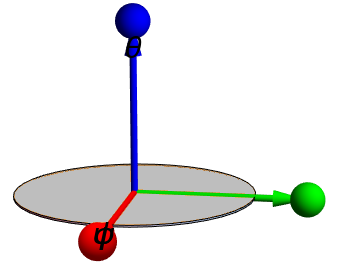
\includegraphics[scale=0.345]{initial}\label{fig:init}}%
	\qquad
	\subfloat[Rotation by $\phi$ about the $z$-axis (blue)]{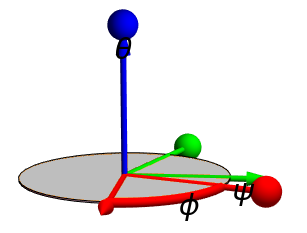
\includegraphics[scale=0.4]{phi_rotation}\label{fig:phirot}}%
	\\
	\subfloat[Rotation by $\theta$ about the new $x$-axis (red)]{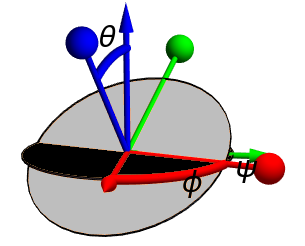
\includegraphics[scale=0.4]{theta_rotation}\label{fig:thetarot}}%
	\qquad
	\subfloat[Rotation by $\psi$ about the new $z$-axis (blue)]{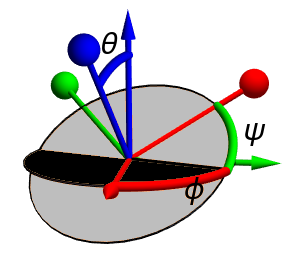
\includegraphics[scale=0.4]{psi_rotation}\label{fig:psirot}}
	\caption{\cite{strauch} \cite{goldstein} Rotation by Euler Angles}
	\label{eulerang}
\end{figure}

 As a demonstration, observe Figure \ref{eulerang} in which we have the Euler angles $\phi, \theta$ and $\psi$. Initially in \ref{fig:init}, we have the principal axes $x$ (red), $y$ (green) and $z$ (blue), each shown as arrows. We then rotate by an angle $\phi$ about the $z$-axis (blue) in \ref{fig:phirot}. Notice that as the rotation by the angle $\phi$ takes place, the $x$ (red) and $y$ (green) axes are displaced but remain perpendicular to $z$ and to each other. The displaced axes (each shown as a ball) now form a new set of principal axes from which we can then perform the next rotation in \ref{fig:thetarot}. 

 \begin{figure}[H]
 	\centering
	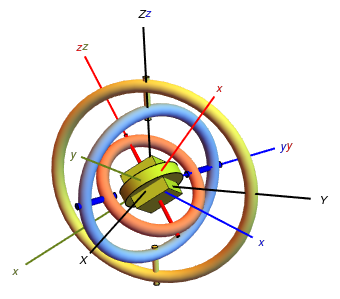
\includegraphics[scale=0.5]{gyro}
 	\caption{Gyroscope}
 	\label{gyroscope}
 \end{figure}

 Alternatively, we can visualize a rotation using a \emph{gyroscope} as seen in Figure \ref{gyroscope} where rotations about the $x$, $y$, and $z$ axes are represented by the red, yellow, and blue rings respectively.
 
 Computing for the image of a point in $\R^3$ under a rotation using Euler angles requires $4\times 4$ matrices like the ones shown in Figure \ref{4x4}. 
\begin{figure}[h]
	\begin{align*}
			\Rx{R}{x}{\alpha} &=
			\begin{pmatrix}
				1 & 0 & 0 & 0 \\
				0 & \cos{\alpha} & -\sin{\alpha} & 0 \\
				0 & \sin{\alpha} & \cos{\alpha} & 0 \\
				0 & 0 & 0 & 1
			\end{pmatrix}
			&
			\Rx{R}{y}{\beta} &=
			\begin{pmatrix}
				\cos{\beta} & 0 & \sin{\beta} & 0 \\
				0 & 1 & 0 & 0 \\
				-\sin{\beta} & 0 & \cos{\beta} & 0 \\
				0 & 0 & 0 & 1
			\end{pmatrix} \\
			(a) & \text{Rotation by $\alpha$ in the x-axis} 
			& 
			(b) & \text{Rotation by $\beta$ in the y-axis}	
	 \end{align*} 
		 \begin{align*}
			\Rx{R}{z}{\gamma} &=
			\begin{pmatrix}
				\cos{\gamma} & -\sin{\gamma} & 0 & 0 \\
				\sin{\gamma} & \cos{\gamma} &  0 & 0 \\
				0 & 0 & 1 & 0 \\
				0 & 0 & 0 & 1
		 \end{pmatrix} \\
		 (c) & \text{Rotation by $\gamma$ in the z-axis}	
		\end{align*}
		\caption{$4\times 4$ Rotation Matrices about the Principal Axes}
		\label{4x4}
\end{figure}

We can rotate any vector/point $\vec{v} \in \R^3$ by matrix multiplication $\pvec{v}' = \Rx{R}{x}{\alpha}\Rx{R}{y}{\beta}\Rx{R}{z}{\gamma}\vec{v}$. However, these computations are a bit tedious and require more elementary arithmetic operations \cite{lerios}. It's also more difficult to determine the axis and angle of rotation \cite{lerios}. Furthermore, this method is susceptible to a problem in mechanics known as the \emph{Gimbal Lock} \cite{jia}.

The gimbal lock is a phenomenon that occurs when two successive rotations are about the same axis as seen in \ref{fig:phigimbal} \cite{goldstein}. This means that a rotation described by $\phi$ can be described by $\psi$ too. We, therefore, have a variable that depends on another, i.e., a variable that can no longer vary independently. This indicates a loss of one degree of freedom. 

\begin{figure}[H]
\centering
\subfloat[A rotation by $\phi$ then $\psi$ about the same axis.]{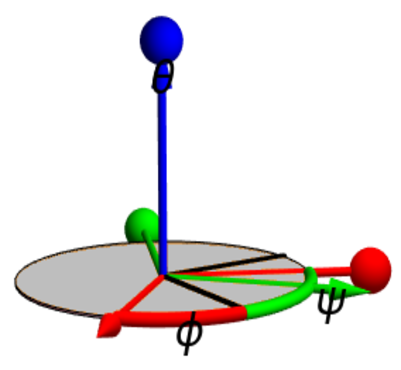
\includegraphics[scale=0.4]{gimbalLockrot}\label{fig:phigimbal}}%
\qquad
\subfloat[The blue and yellow rings coincide resulting in a loss of one degree of freedom.]{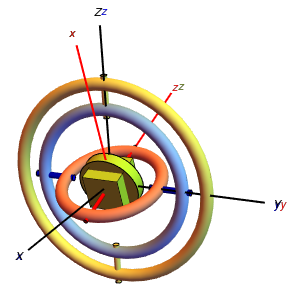
\includegraphics[scale=0.5]{gimbalLock}\label{fig:lock}}
\caption{The Gimbal Lock}
\label{gimbal}
\end{figure}

The same is true for the gyroscope example in \ref{fig:lock} in which two of the rings coincide (yellow and blue). A rotation described by the red ring can also be described by the outer yellow ring. In other words, the outer rings have "locked" the rotations described by the red ring.

There is a simpler and more elegant way to describe three-dimensional rotation which involves the algebra of \emph{Quaternions} (discovered by Rowan Hamilton in 1843). Using quaternions, one only needs to specify the angle of rotation and a three-dimensional vector about which a point in space rotates (axis of rotation). 

One can write a quaternion as an ordered pair $(a,\vec{v})$ where $a$ is a scalar, and $\vec{v}$ is a three-dimensional vector \cite{mathoma}. In order to rotate a point/vector $\vec{v} \in \R^3$ about a unit vector $\vec{u_1}$ (axis of rotation), we first need to write $\vec{v}$ as a quaternion $p = (0,\vec{v})$. We then perform a conjugation on $p$ by a quaternion $q$,i.e., $p' = qpq^{-1}$ where $q = (\text{cos}(\frac{\theta}{2}),\vec{u_1} \text{sin}(\frac{\theta}{2}))$ \cite{balmens2}. The vector part of the resulting quaternion $p'$ is the vector obtained after the rotation about $\vec{u_1}$ by an angle $\theta$. 

\begin{figure}[t]
	\centering
	\subfloat[Rotation about the $z$-axis]{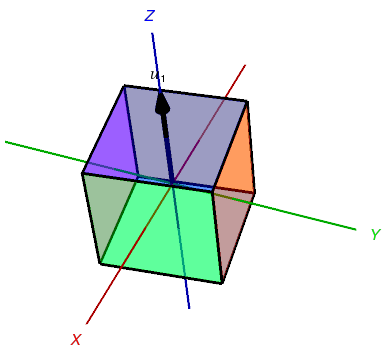
\includegraphics[scale=0.5]{quatzrot}\label{fig:quatzrot}}%
	\qquad
	\subfloat[Rotation about some axis]{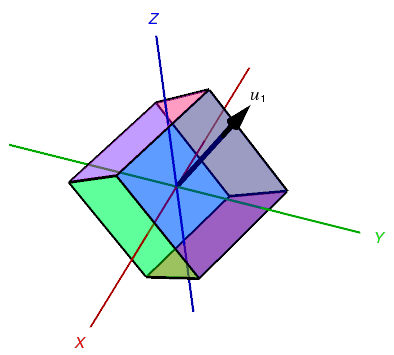
\includegraphics[scale=0.5]{arbrot}\label{fig:arbrot}}
	\caption{\cite{balmens2} Rotation using the quaternion $(0,\vec{u_1})$}
	\label{quatrot}
\end{figure}

Because quaternions do not require rotations about principal axes to describe three-dimensional rotation, quaternions do not suffer from the gimbal lock. They are also found to be more compact - requiring less elementary arithmetic operations to perform rotation composition than rotation matrices \cite{lerios}. 

Quaternions are used today in robotics, three-dimensional computer graphics, computer vision, crystallographic texture analysis, navigation, and molecular dynamics. 

Mathematicians have made advancements in developing the theory of Quaternions. Notably, as one of the central points of this topic, we look into the concept of a \emph{Quaternionic Matrix} and the implications it has on certain definitions that were already established in Linear Algebra. 

One such implication is the concept of a determinant in the context of quaternionic matrices. In linear algebra, we saw that we can extend the definition of the determinant to matrices with complex entries \cite{stamaria}. This is possible because the complex numbers are commutative under complex multiplication \cite{aslaksen}. 

Certain problems arise if we attempt to extend the classical definition to the quaternions because quaternions are not commutative under quaternion multiplication \cite{aslaksen}. In \cite{aslaksen}, the following properties we associate with determinants are revisited and three conditions called \emph{axioms} are given that should be satisfied in order for a definition of a determinant to be valid and useful:
\begin{itemize}
	\item \textbf{Axiom 1} $det(A) = 0$ if and only if $A$ is singular.
	\item \textbf{Axiom 2} $det(AB) = det(A)det(B)$ for all quaternionic matrices $A$ and $B$.
	\item \textbf{Axiom 3} If $A'$ is obtained by adding a left-multiple of a row to another row or a right-multiple of a column to another column, then $det(A')=det(A)$.
\end{itemize}

Over the years, several mathematicians have come up with different ways to define a determinant for quaternionic matrices - the Cayley determinant (by Arthur Cayley in 1845), the Study determinant (by Eduard Study in 1920), the Dieudonne determinant, and Moore's determinant. Aslaksen showed whether or not the Cayley, Study, Dieudonne, and Moore's determinant satisfy the axioms \cite{aslaksen}.

In this paper, we will discuss the theory behind quaternionic linear maps and quaternionic determinants - particularly, the Study determinant. 
\iffalse
We will then use the Study determinant to extend a result in \cite{stamaria} to the set of all skew-coninvolutory quaternionic matrices, i.e., we will show that the set of all $n \times n$ skew-coninvolutory quaternionic matrices is empty when $n$ is odd. 
\fi
\newpage
\section{List of Symbols}

\begin{itemize}
	\item $\Mr{n}$ - set of all $n\times n$ matrices with real entries.
	\item $\Mc{n}$ - set of all $n\times n$ matrices with complex entries.
	\item $\Mh{n}$ - set of all $n\times n$ matrices with quaternion entries.
	\item $\mathscr{D}_n(\CC)$ - set of all $n\times n$ skew-coninvolutory matrices with complex entries.
	\item $\mathscr{D}_n(\HH)$ - set of all $n\times n$ skew-coninvolutory matrices with quaternion entries.
	\item $\cdet{ }$ - determinant of a matrix in $\Mc{n}$.
	\item $\rdet{ }$ - determinant of a matrix in $\Mr{n}$.
\end{itemize}